\section{A theoretical framework for multi-modal learning}
\label{sec::framework}

As outlined in the Introduction, we assume that there exists a mapping between (sets of) patterns belonging to different modalities --- here we focus upon the relations which exist between a passive and an active modality. In the aforementioned example dealing with objects (as seen) and grasping them, something like what is shown in Figure \ref{fig::implementation} is sought for.

\begin{figure}[h!]
	\centering
	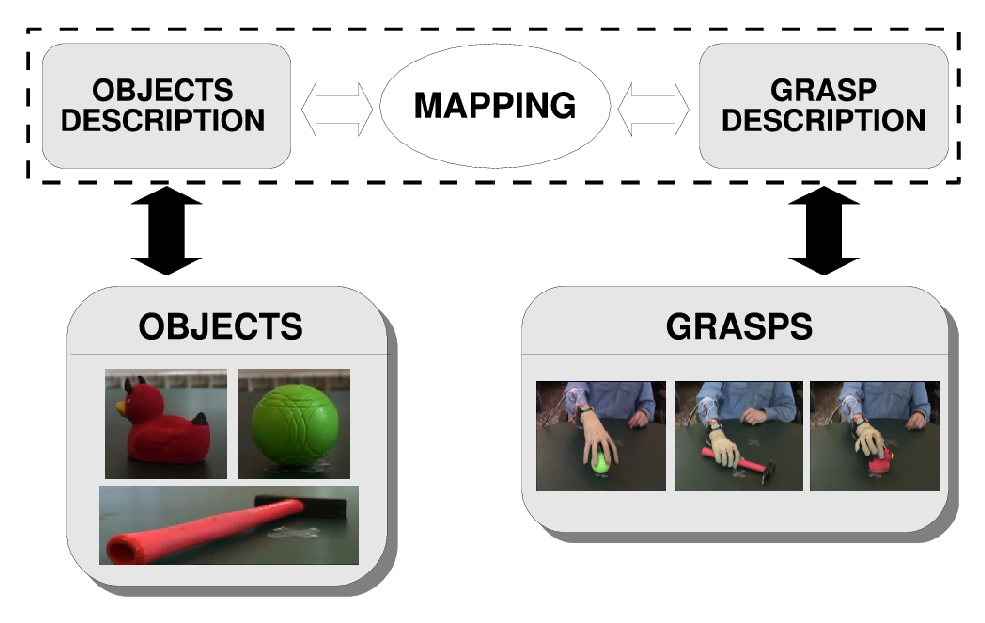
\includegraphics[width=0.7\textwidth]{images_pdf/images/schema_implementazione}
	\caption{An instance of the framework we propose: estimating a
     mapping between appropriate visual descriptions of objects and
     classes of grasp actions. For the time being, we assume that such
     relation is a one-to-one mapping.}
	\label{fig::implementation}
\end{figure}
%\vskip -0.5cm

In general, active modalities are not available to a biological system during the prediction phase, but only during the training phase. A paradigmatic example is that of a human infant learning how to grasp an object: by repeatedly trying to apply, e.g., a cylindric grasp to a bottle, he will learn not only to do it more and more efficiently, but also that a bottle is better be grasped cylindrically when moving it or bringing it close to the mouth. Later on, the sight of a bottle will remind the young human what one of the correct grasps is for that particular object. 
A \emph{perception-to-action map} (PAM) is the equivalent of such training for a biological system: a model to reconstruct an active modality from a passive one. The PAM of our example is a mapping from visual features of an object to motor features of the grasping action used for that object. In general such a map is many-to-many: both a hammer and a bottle can be grasped cylindrically\footnote{The nomenclature of grasp types loosely follows that of Cutkosky \cite{cutkosky}.}), and as well a mug can be handled either cylindrically or by the handle. In this work we make the simplifying assumption that for a specific object there is just one acceptable grasping action --- the PAM is one-to-one.
A PAM is useful in passive pattern recognition (e.g., classifying an object just by seeing it) since it augments the input space with PAM-reconstructed active patterns (e.g., classifying the same object from its sight \emph{and the associated grasp}). In this preliminary work we focus upon a simpler problem, namely that of checking whether, given the visual features of an object, the PAM-reconstructed grasp is (similar to) the one associated with that particular object. For example, we might train a PAM to reconstruct a pinch grip (hand posture) from the visual features of a pen; given then, in the prediciton phase, the visual features of another pen, will the PAM-reconstructed hand posture of a pinch grip look like a true pinch grip?



In particular, what is needed is: $(i)$ a \emph{vision unit} to extract visual features from an image or a series of images, and $(ii)$ a \emph{regression unit}, which will build the PAM.

